\documentclass[11pt]{article} % use larger type; default would be 10pt
\usepackage{amsmath}
\usepackage{circuitikz}
\usepackage{tikz}
\usepackage{geometry} % to change the page dimensions
\geometry{a4paper} % or letterpaper (US) or a5paper or....
\geometry{margin=1in}
\usepackage{amssymb}
\usepackage{textcomp}
\usepackage{fancyhdr} % This should be set AFTER setting up the page geometry
\pagestyle{fancy} % options: empty , plain , fancy
\renewcommand{\headrulewidth}{0pt} % customise the layout...
\lhead{ES335}\chead{Lecture 1}\rhead{07/01/2013}
\lfoot{}\cfoot{\thepage}\rfoot{Olly Levett}


\begin{document}
\section{Lecture \ref{sec:lec1} - Modulation}
\label{sec:lec1}
\begin{equation}
	f(t) = \underbrace{A_c}_{\mbox{\scriptsize Amplitude}} \times \cos(\overbrace{\omega}^{\mbox{\scriptsize Angular frequency}} t + \underbrace{\phi _c}_{\mbox{\scriptsize Phase term}})
\end{equation}

Modulation is the process of applying information to a carrier, in this case, the carrier frequency is $\omega _c$ (as an angular frequency) or $f_c$ as a frequency directly where $\omega_c = 2 \pi f_c$.

If we modify $A$ in the above in sympathy with the information we want to send, then this is amplitude modulation.

If however we change $\omega_c$ or $\phi _c$ in sympathy with the information, these are forms of angle modulation - varying $\omega _c$ is frequency modulation, varying $phi _c$ is phase modulation.

If the amplitude etc, varies linearly with the information then this is analogue, alternatively varying these quantities in an on/off manner or between two state is digital.

\subsection{Amplitude Modulation}
The function $f(t)$ becomes
\begin{equation}
	f(t)=\underbrace{A_0(1-m \cos \omega_m t)}_{A} \times \underbrace{cos \omega _0 t}_{\mbox{\scriptsize No $\phi _c$ term}}
\label{eqn:am}
\end{equation}

$f_m$ or ($\omega_m = 2 \pi f_m$) is a simple sine/cosine wave modulation function

Expanding $f(t)$:-
\begin{eqnarray}
f(t) &=A_0 \cos \omega_0t + A_0m \cos\omega_mt x \cos \omega_0 t \nonumber \\
&= A_0 \cos\omega_0t+\frac{A_0m}{2} \cos(\omega_m+\omega_0)t+\cos(\omega_0-\omega_m)t
\end{eqnarray}
	\begin{figure}[h]
		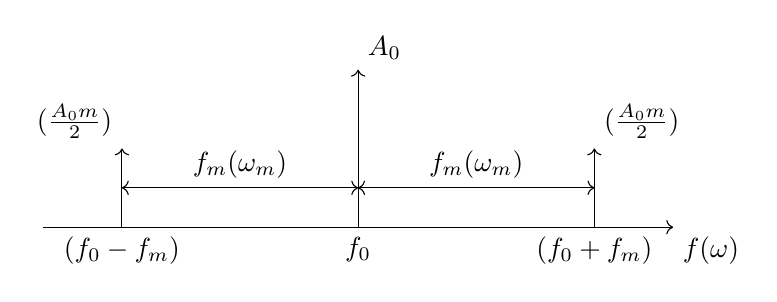
\begin{tikzpicture}
			\draw[->] (1,0) node [below]{$(f_0-f_m)$} -- (1,1) node [above left] {$(\frac{A_0m}{2})$};
			\draw[->] (7,0) node [below]{$(f_0+f_m)$} -- (7,1) node [above right] {$(\frac{A_0m}{2})$};
			\draw[->] (4,0) node [below]{$f_0$} -- (4,2) node [above right] {$A_0$};
			\draw[->] (0,0) -> (8,0) node [below right] {$f(\omega )$};
			\draw[<->] (1,0.5)--(4,0.5);
			\node[align=center, above] at (2.5,0.5) {$f_m(\omega_m)$};
			\node[align=center, above] at (5.5,0.5) {$f_m(\omega_m)$};
			\draw[<->] (7,0.5)--(4,0.5);
		\end{tikzpicture}
		\centering
		\caption{Spectrum of an AM signal, including sidebands}
	\end{figure}

% $A_0$ contains no useful information (bar frequency) which is a disadvantage of Amplitude Modulation.

The simple process of amplitude modulation produces an upper sideband (USB) at $f_0+f_m$ and a lower sideband at $f_0-f_m$. Note that only the sidebands contain any useful information about the amplitude $m$ of the modulation signal.

This modulation has a power penalty because the carrier conveys no useful amplitude information itself.
\begin{eqnarray}
\left(\frac{\mbox{Power in sidebands}}{\mbox{Total power transmitted}}\right) &=& \frac{(0.5A_0m)^2+(0.5A_0m)^2}{(0.5A_0m)^2+(0.5A_0m)^2+A_0^2} \nonumber \\
&=& \frac{0.5A_0^2m^2}{0.5A_0^2m^2 + A_0^2} \nonumber \\
&=& \frac{0.5m^2}{0.5m^2+1}
\label{eqn:power}
\end{eqnarray}

$m = \mbox{modulation depth} = \left(\frac{A_m}{A_0}\right)$ which is a ratio of modulation voltage to the carrier voltage (or current).

It is essential not to let $|m|\ge 1$ because this is overmodulation and it distors the AM waveform.

Going back to equation \ref{eqn:power}  in the limit $m=1$ and so the ratio is:-
\begin{equation}
\frac{0.5\times 1^2}{(0.5\times 1^2)+1} = \frac{0.5}{1.5} = \frac{1}{3} = 33.3\%
\end{equation}
$\frac{2}{3}$ of the transmitted power is wasted.

Typically, $m\approx 4$ from which we have:-
\begin{equation}
\frac{0.5\times 0.4^2}{(0.5\times 0.4^)+1} = \frac{0.08}{0.08+1}
\end{equation}
so this ratio is around 0.08 ie. only 8\% of the transmitted power is used, or 92\% is wasted!

\subsubsection{Waveforms}
	\begin{figure}[h]
		\centering
		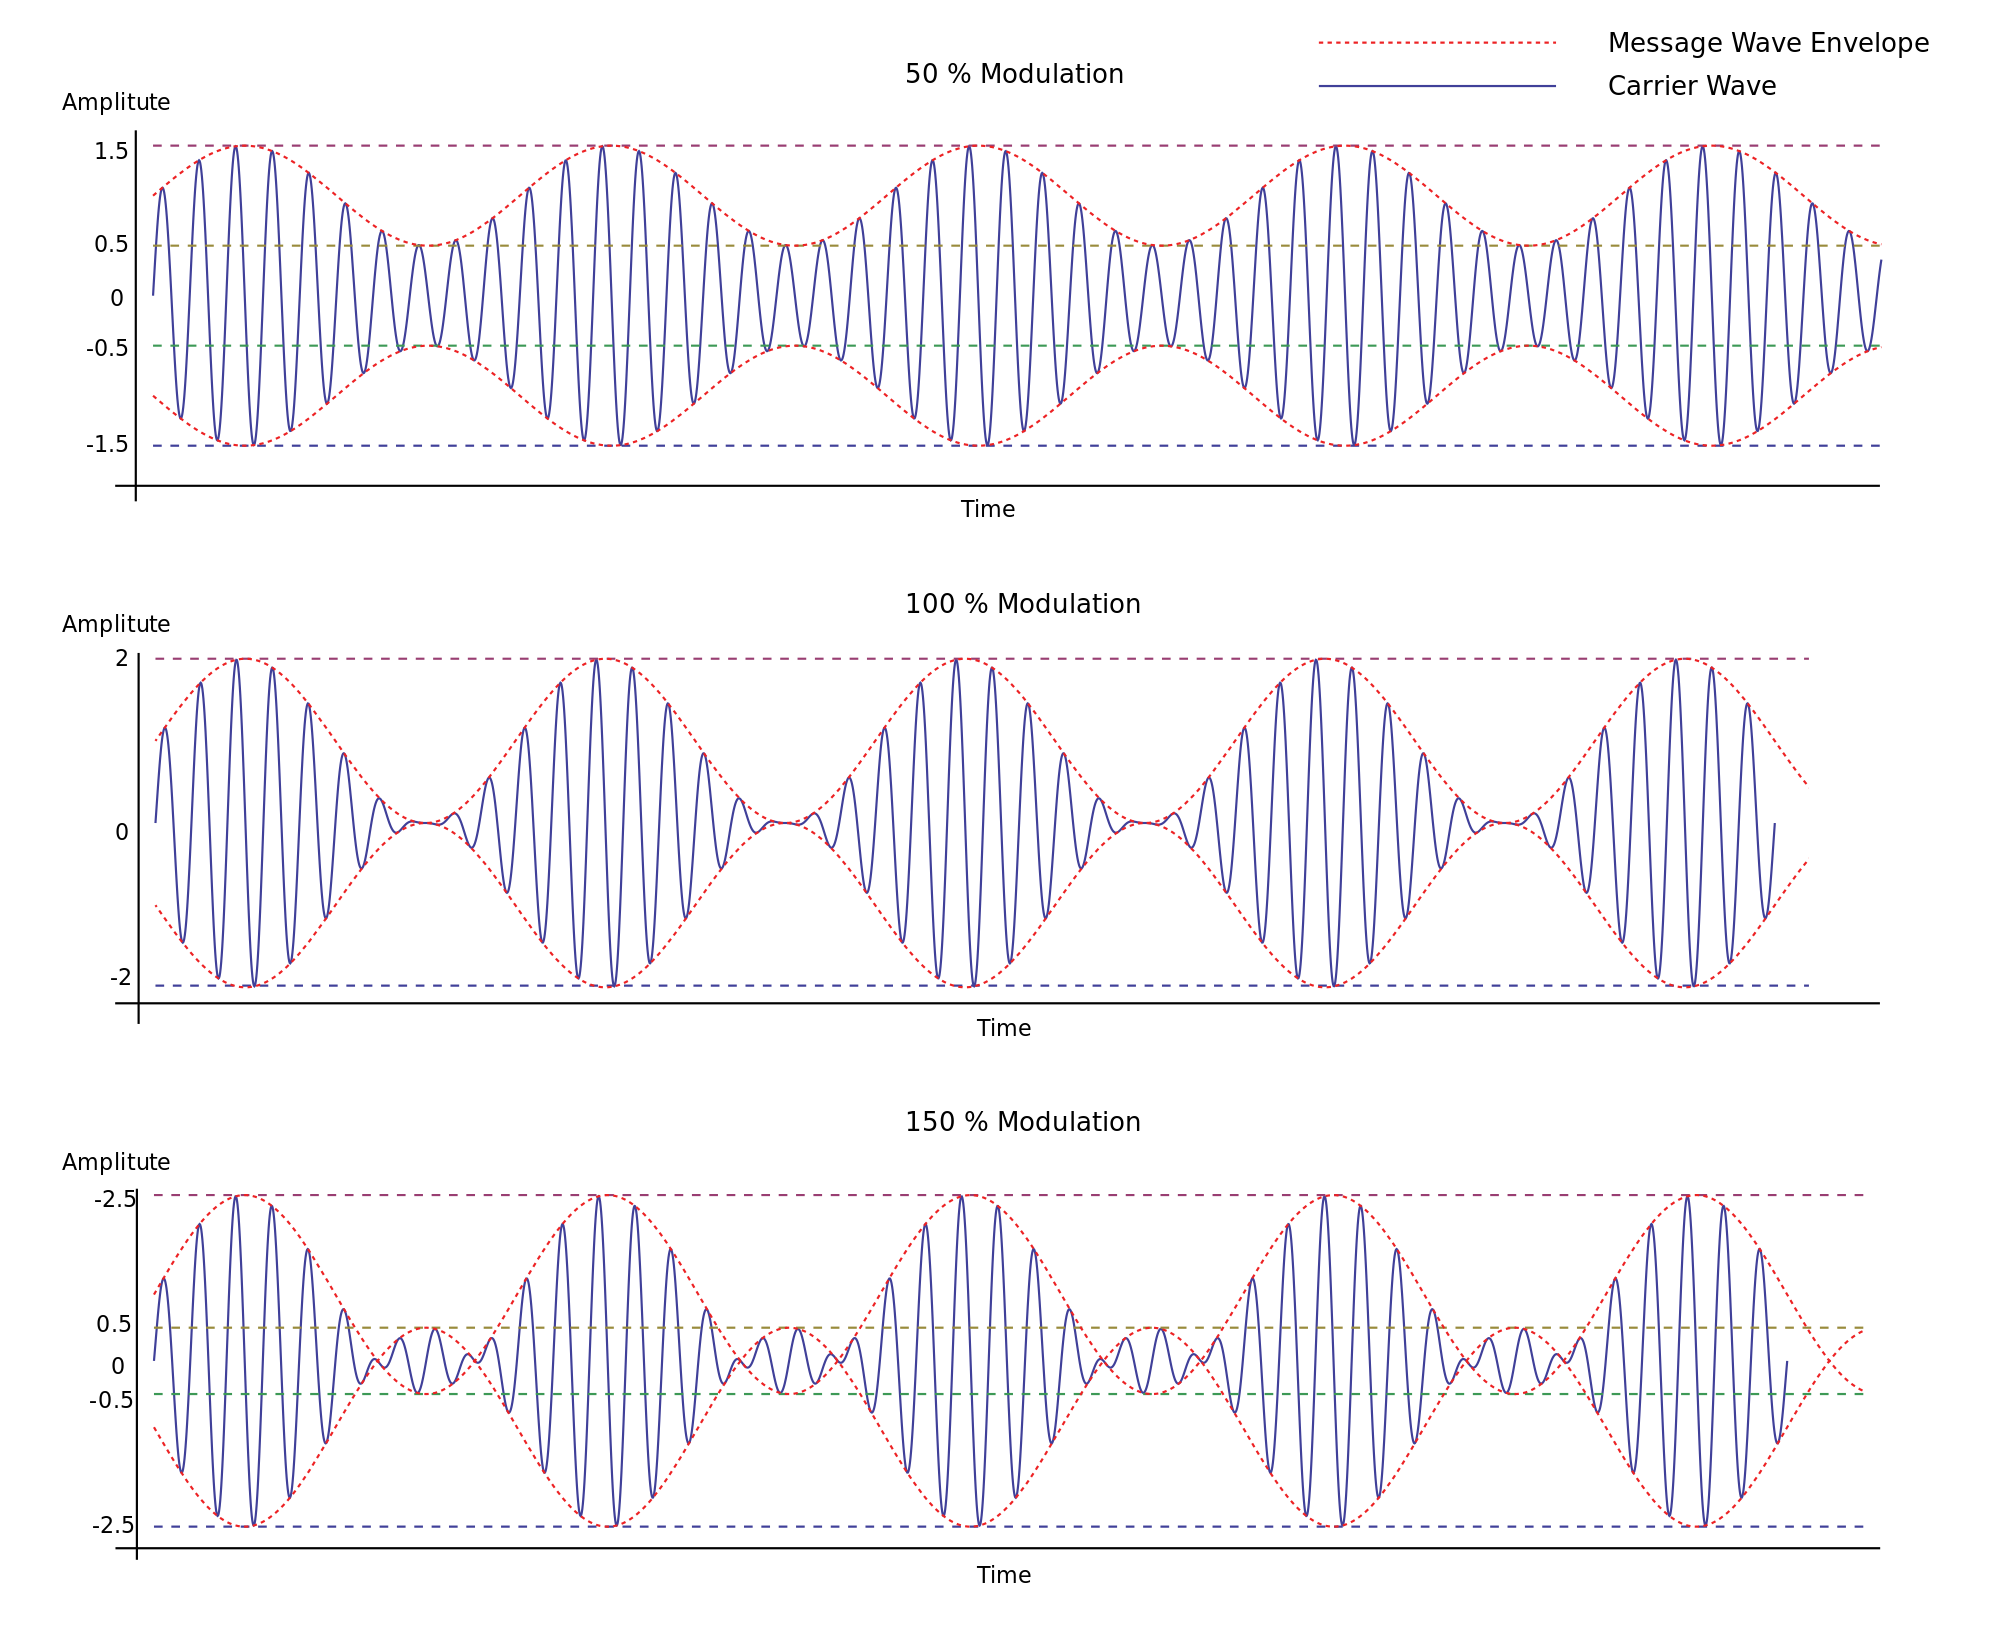
\includegraphics[width=0.8\textwidth]{modulatedwave}
	\end{figure}
It is essential, when considering the above waveform, to have $|m|\le 1$ as mentioned before.

Detecting AM requires an envelope detector in its simplest form:-

\begin{figure}[h]
\centering
\begin{circuitikz}
	\draw
	(0,2) node[anchor=east]{AM input}
	to[D*,o-*] (3,2)
	to[R, l=$R_L$,*-*] (3,0);
	\draw (0,0) to [short,o-*] (3,0);
	\draw (3,2) to[short, *-o] (5.5,2);
	\draw (3,0) to[short, *-o] (5.5,0);
\end{circuitikz}
\end{figure}

A more advanced envelope detector adds a low pass filter to remove high frequency components from the carrier wave.
\begin{figure}[h]
\centering
\begin{circuitikz}
	\draw
	(0,2) node[anchor=east]{AM input}
	to[D*,o-*] (3,2)
	to[R, l=$R_L$,*-*] (3,0)
	to[short,*-o] (0,0);
	\draw (3,2) to[short, *-o] (7.5,2);
	\draw (3,0) to[short, *-o] (7.5,0);
	\draw (5.5,0) to[C,*-*] (5.5,2);
\end{circuitikz}
\end{figure}

If the carrier frequency is high compared to the modulation frequency, the recovered envelope is a "quite good" approximation to the original given a certain combination of $R_L$ and $C$.

\section{Lecture \ref{sec:lec2} - }
\label{sec:lec2}
\subsection{Double Sideband and Single Sideband AM}
Recall AM signal (Equation \ref{eqn:am})

Power is wasted in carrier, so a better form of A.M. could be:-
\begin{equation}
f(t) = A_0 \times \cos{\omega_0} \times m\cos{\omega_m t}
\end{equation}
Where $m=\frac{A_m}{A_0}$ = modulating depth
$A_m$ = amplitide of mudlationg signal

\begin{equation}
f(t) = \left(\frac{A_0m}{2}\right)
\left(\cos{(\omega_0  \omega_m)}t+\cos{(\omega_0 - \omega_m)}\right)
\end{equation}

This is known as double sided sideband, supressed carrier (DSB).

There is an important property of a DSB $\rightarrow$ for no modulation, no signal is sent, so that it is very power effiicient, but not badnwidth efficient.

\begin{figure}[h]
		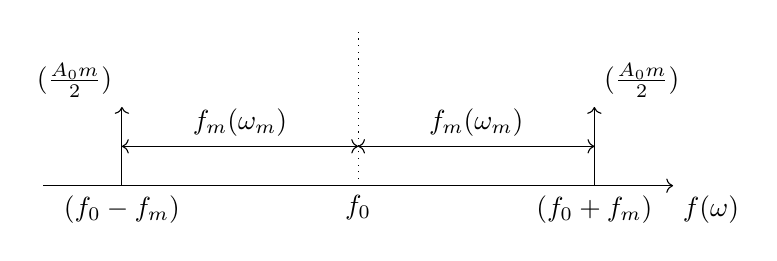
\begin{tikzpicture}
			\draw[->] (1,0) node [below]{$(f_0-f_m)$} -- (1,1) node [above left] {$(\frac{A_0m}{2})$};
			\draw[->] (7,0) node [below]{$(f_0+f_m)$} -- (7,1) node [above right] {$(\frac{A_0m}{2})$};
			\draw[dotted] (4,0) node [below]{$f_0$} -- (4,2);
			\draw[->] (0,0) -> (8,0) node [below right] {$f(\omega )$};
			\draw[<->] (1,0.5)--(4,0.5);
			\node[align=center, above] at (2.5,0.5) {$f_m(\omega_m)$};
			\node[align=center, above] at (5.5,0.5) {$f_m(\omega_m)$};
			\draw[<->] (7,0.5)--(4,0.5);
		\end{tikzpicture}
		\centering
		\caption{Spectrum of an AM signal, including sidebands}
	\end{figure}


The envelope of a DSB signal for a single frequency of modulation is:-
\begin{figure}[h]
	\begin{tikzpicture}
		\draw[->] (0,0)--(6.28,0);
		\draw (0,0) -- (6.28,6.28);
		\draw[color=red,domain=0:6.28,samples=200,smooth] plot (\x,{sin(\x)});
	\end{tikzpicture}
\end{figure}

Because there is no carrier present, the envelope of the DSB waveform no longer represents the modulating function, therefore an envelope detector cannot be used to detect it - a product detector is used instead.

To illustrate the operation, instead of a DSB being the input, simply use a carrier frequency with no modulation



The output after filtering is $\left(\frac{A_0E}{2}\right)$ which is proportinal to $A_0$, the signl amplitude.

Replace the simple input by:-
\begin{equation}
A_0\cos{\omega_0 t} \times \cos{\omega_m t}
\end{equation}
output is
\begin{eqnarray}
(A_0 \times \cos{\omega_t} \times \cos{\omega_m t})(E\times\cos{\omega_0 t})
&=& A_0 E \cos^2{\omega_0 t}\times\cos{\omega_m t} \\
&=& \left(\frac{A_0 E}{2}\right)(1+\cos{2 \omega_0 t}) \times \cos{\omega_m t}
\end{eqnarray}

After low pass filtering to remove all frequences above $\omega_m$:-
\begin{equation}
OP = \left(\frac{A_0 E}{2}\right) \times \cos{\omega_m t}
\end{equation}which represent the modulation function directly.

This sustem can be improved even further because bandwidth is wasted. Bandwith is important because it is a scarce resources.

If we consider the expanded form of that for DSB:-
\begin{equation}
f(t) = \left(\frac{A_0m}{2} \right) \cos{\left(\omega_0 + \omega_m\right)}t + \left(\frac{A_0m}{2} \right)  \cos{\left(\omega_0 - \omega_m\right)}t 
\end{equation}
If we filter carfully, then we need only send either the USB or LSB.

% Filter image...

Filtering therefore reduces the badnwidth, as each sideband carries the same information (each has an "m" term). Difficulty arrises in obtaining sharp cuttof filters. The PHASING METHOD can be used to generate SSB (single side band).

% SSB diagram

\begin{equation}
E_0 = E_1+E_2
\end{equation}

\begin{eqnarray}
E_1 &=& \left[ A_0 \cos{\omega_0 t}\right] \times \left[ \cos{\omega_m t + \frac{\pi}{2}}\right]\nonumber \\
&=& A_0 \cos{\omega_0t}\times \sin{\omega_m t}
\end{eqnarray}

$\therefore$
\begin{equation}
E_2 = A_0 \sin{\omega_0t}\times \cos{\omega_m t}
\end{equation}

$\therefore$
\begin{eqnarray}
E_0 &=& A_0 \times \left[\cos{\omega_0t}\times \sin{\omega_m t}+  \sin{\omega_0t}\times \cos{\omega_m t}\right] \nonumber \\
&=& A_0 \sin{\left(\omega_0 + \omega_m\right)} t
\end{eqnarray}
USB, no filtering needed.

Similarly, the LSB can be generated by changing the sign of the second term above (on the first term).

The method works very well only when a single frequency of modulation is used. In practise, a range of frequences is used and it is very difficult to obtain a 90\textdegree phase shift over a range of frequencies.

\subsection{Vestigial Sideband}
Rememober the abbrs, "in case they get slipped into a question"
This is an approximation to SSB which has been used extensively in analoge T.V. ver many decades. Basically, a DSB/C (Double Sideban with Carrier)

% Vestigial sideband sign...

The main benefits are: simplicty and cheapness compared to SSB, when using valve/vacuum tube technologies.

The disadvantage is carrier still there, wasting power, but alowing an envelope detector (cheap, easy to make) to be used.
\end{document}